\section*{Bài 4}

Giải hệ phương trình đồng dư sau:
$$ \begin{cases}
    x \equiv 2 \Mod{5}\\
    x \equiv 5 \Mod{9}\\
    x \equiv 8 \Mod{11}\\
    x \equiv 13 \Mod{13}
\end{cases} $$
	
\addcontentsline{toc}{section}{Bài 4}

\centering
\textbf{\underline{Bài làm:}}

\justifying
Để giải hệ phương trình đồng dư tuyến tính, ta sẽ sử dụng định lí số dư Trung Hoa.

\textbf{Mã giả của thuật toán:}\\
\begin{algorithm}[H]
\setstretch{1.15}
\renewcommand{\algorithmcfname}{Thuật toán}

\caption{Giải hệ phương trình đồng dư sử dụng định lí số dư Trung Hoa}
\SetKwFunction{len}{len}
\SetKwFunction{Remove}{Remove}
\SetKwFunction{Multiply}{Multiply}
\SetKwFunction{ExtendedGCD}{ExtendedGCD}
\SetKwInOut{Input}{Đầu vào}\SetKwInOut{Output}{Đầu ra}
\SetAlgoNoEnd\SetAlgoNoLine%

\Input{$a = \big( a_1, a_2, ..., a_k \big)$ là $k$ số nguyên tùy ý và $k$ số nguyên dương đôi một nguyên tố cùng nhau $m = \big( m_1, m_2, ..., m_k \big)$. Khi đó ta có hệ phương trình đồng dư tuyến tính sau:
$$ \begin{cases}
    x \equiv a_1 \Mod{m_1}\\
    x \equiv a_2 \Mod{m_2}\\
    \vdots\\
    x \equiv a_k \Mod{m_k}
\end{cases} $$
}
\Output{2 số nguyên dương $b, c$ sao cho $x \equiv b \Mod{c}$ là nghiệm của hệ trên.}
$S \leftarrow 0$\\
$N \leftarrow 0$\\
$N^{-1} \leftarrow 0$\\
$b \leftarrow 0$\\
\For{$i \leftarrow 1$ \KwTo $\len(a)$}{
    \tcc{Hàm Remove dùng để loại bỏ phần tử thứ i trong a}
    $S \leftarrow \Remove(a, i)$\\
    \tcc{Hàm Multiply dùng để tính tích các phần tử trong S}
    $N \leftarrow \Multiply(S)$\\
    \tcc{Lấy nghịch đảo module sử dụng thuật toán Euclid mở rộng trong bài 3c}
    $N^{-1} \leftarrow \ExtendedGCD(N, m_i)$\\
    $b \leftarrow b + a_i \cftdot N \cftdot N^{-1}$
}
\Return $b, \Multiply(m)$
\end{algorithm}

\textbf{Giải tay:}

Ta có:
\begin{ceqn}
\begin{align*}
N_1 &= 9 \cftdot 11 \cftdot 13 = 1287 \equiv 2 \Mod{5} \Rightarrow N_1^{-1} = 3\\
N_2 &= 5 \cftdot 11 \cftdot 13 = 715 \equiv 4 \Mod{9} \Rightarrow N_2^{-1} = 7\\
N_3 &= 5 \cftdot 9 \cftdot 13 = 585 \equiv 2 \Mod{11} \Rightarrow N_3^{-1} = 6\\
N_4 &= 5 \cftdot 9 \cftdot 11 = 495 \equiv 1 \Mod{13} \Rightarrow N_4^{-1} = 1
\end{align*}
\end{ceqn}

Vậy nghiệm của hệ phương trình là:
$$x = 2 \cftdot 1287 \cftdot 3 + 5 \cftdot 715 \cftdot 7 + 8 \cftdot 585 \cftdot 6 + 13 \cftdot 495 \cftdot 1 = 67262 \equiv 2912 \Mod{5 \cftdot 9 \cftdot 11 \cftdot 13 = 6435}$$

\textbf{Hiện thực thuật toán trên Maple:}

Ta định nghĩa thủ tục (procedure) $\mathtt{ChineseRemainder} \big( a, m \big)$ như trong hình bên dưới. Sau đó, ta chạy thử thuật toán tìm nghiệm của 2 hệ phương trình đồng dư sau:
$$ \begin{cases}
    x \equiv 2 \Mod{3}\\
    x \equiv 3 \Mod{5}\\
    x \equiv 5 \Mod{7}
\end{cases} \quad \big( 1 \big) $$
và
$$ \begin{cases}
    x \equiv 6 \Mod{11}\\
    x \equiv 13 \Mod{16}\\
    x \equiv 9 \Mod{21}\\
    x \equiv 19 \Mod{25}
\end{cases} \quad \big( 2 \big) $$

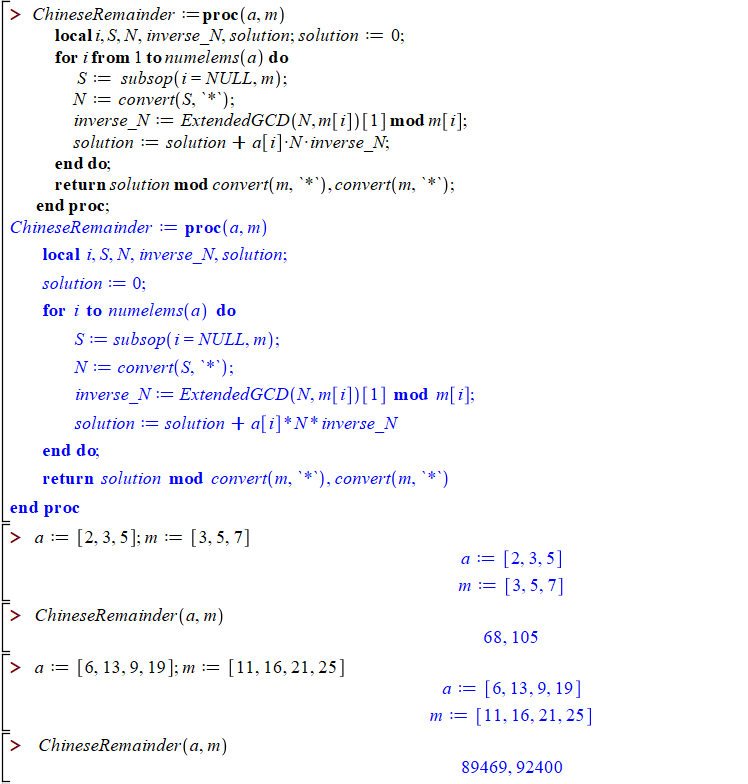
\includegraphics[width=1.0\textwidth]{bai4_maple_euclidean_algorithm.png}

Như vậy ta thấy nghiệm của hệ phương trình $\big( 1 \big)$ là $x \equiv 68\Mod{105}$, nghiệm của hệ phương trình $\big( 1 \big)$ là $x \equiv 89469\Mod{92400}$.

Bây giờ, ta đi tìm nghiệm của hệ phương trình đồng dư của \textbf{bài 4} sử dụng thủ tục (procedure) $\mathtt{ChineseRemainder} \big( a, m \big)$ đã được định nghĩa trong \textbf{Maple} như ở trên.

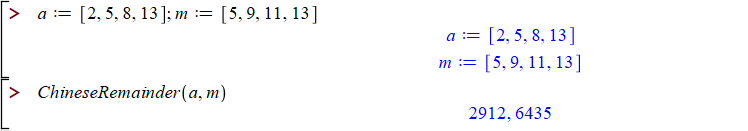
\includegraphics[width=1.0\textwidth]{bai4_maple_answer.png}

Vậy nghiệm của hệ phương trình đồng dư ở \textbf{bài 4} là $x \equiv 2912\Mod{6435}$.
	
\clearpage